
\section{Results and Discussion}
% Describe evaluation methodology and significant results in the evaluation section
% Evaluate the selected approach and analyze why the selected approach is good?
%   Provide an intuitive description of the algorithms, their correctness and their complexity
The simulation was run
on a Dell Laptop with a 11th Gen Intel(R) Core(TM) i7-11800H processor (8 cores, 16 threads)
running at 2.30GHz, 64.0 GB of installed RAM,
a 64-bit operating system with an x64-based processor
using Python3.10 and pytest as the driver.
We selected Pytest because the test-isolation generalizes
well for simulations. Therefore, simulations
are `tests' marked with the \texttt{@pytest.mark.simulation}
marker. Because running a simulation is slow,
these tests are also marked as \textit{slow}.
More importantly, we run our simulation
distributed across multiple CPUs. Given that
each simulation is isolated, we can run
all the simulations in parallel
by using pytest-xdist framework~\cite{pytestXdist}.
Additionally, pytest ships with runtime
tracking out of the box.
Refer to \autoref{fig:simulation}
for an example output of a running simulation.

\begin{figure}[!htp]
    \centering
    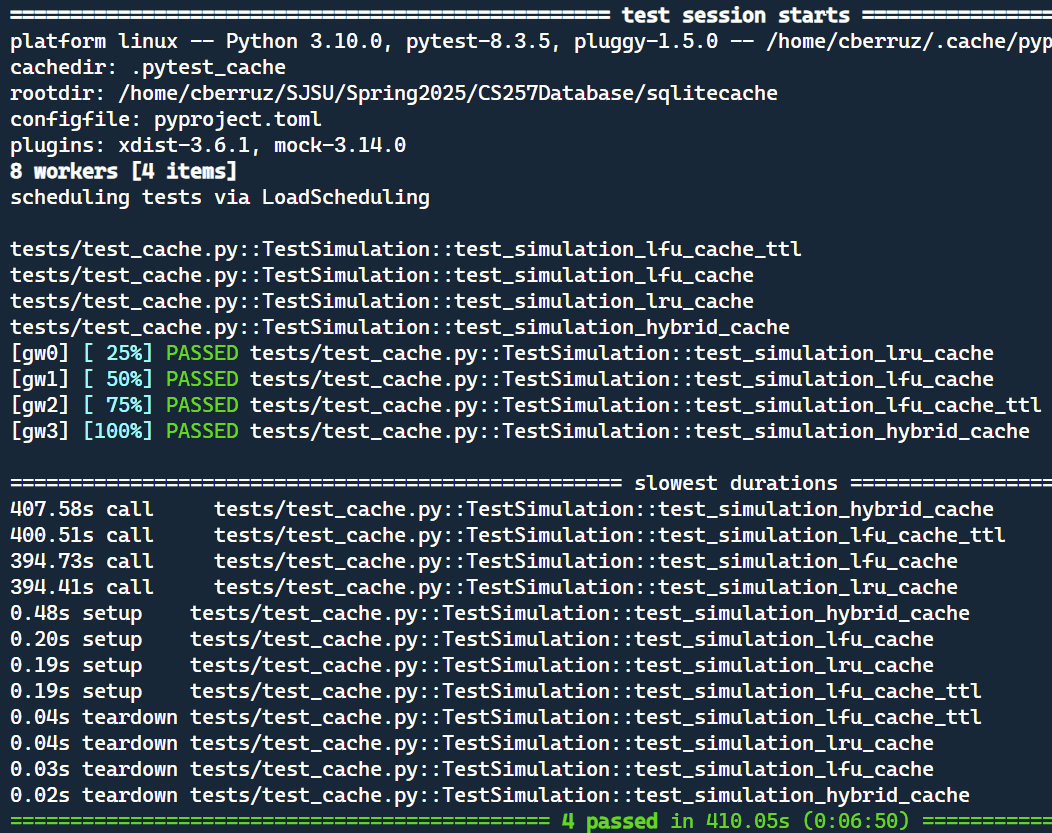
\includegraphics[width=\linewidth]{images/simulation_running_example.png}
    \caption{Screenshot of a running simulation.}
    \label{fig:simulation}
\end{figure}

We let $P = 100$.
In our platform, all uncompressed and unencrypted
values in $D$ occupy $b = 18$ bytes.
Therefore, the cache size $P' = Q' = 1800$ bytes.
Furthermore, no compression and no encryption
was enabled.

The simulation was run as a sustained load,
as described in Algorithm~\ref{alg:simulation}.
This means that it runs until completion
for
$N$ requests. For example, in $N=1000$
we generate 1000 data points for both
the hit and miss rates. The duration
of each simulation run was dependent
on the eviction policy being tested.
TTL based policies, such as LFUCacheTTL
and HybridCache as seen in \autoref{fig:simulation}.

\begin{figure*}[!htp]
    \centering
    \begin{tikzpicture}
        \begin{axis}[
            width=\linewidth*0.9,
            height=8cm,
            xlabel={n\_requests},
            ylabel={hit\_rate},
            grid=major,
            legend style={at={(0.95,0.05)}, anchor=south east},
            title={Hit Rate vs. Number of Requests}
        ]
        \addplot[
            color=blue,
        ] table [
            col sep=comma,
            x={requests},
            y={hit_rate}
        ] {data/LRUCacheSimulationResults.csv};
        \addplot[
            color=red,
        ] table [
            col sep=comma,
            x={requests},
            y={hit_rate}
        ] {data/LFUCacheSimulationResults.csv};
        \addplot[
            color=orange,
        ] table [
            col sep=comma,
            x={requests},
            y={hit_rate}
        ] {data/LFUCacheTTLSimulationResults.csv};
        \addplot[
            color=black,
        ] table [
            col sep=comma,
            x={requests},
            y={hit_rate}
        ] {data/HybridCacheSimulationResults.csv};
        \legend{LRUCache, LFUCache, LFUCacheTTL, HybridCache}
        \end{axis}
    \end{tikzpicture}
    \caption{Hit rate as a function of number of requests for different cache eviction policies.}
    \label{fig:hit_rate_plot}
\end{figure*}

A total of four eviction policies were tested:
LRU, LFU, LFU with TTL, and Hybrid.
The results of the hit rate vs. the number
of request for each eviction policy is summarized
in \autoref{fig:hit_rate_plot}.

It is clear that the HybridCache policy performs significantly
better than all other policies. The LRUCache performs the worst
among all eviction policies. These results
are in alignment with~\cite{shah2023ImprovedCacheEviction}.